TODO: this needs to be organized, could use some figures too.

Motzkin, Schröder, and Łukasiewicz paths provide generalizations of Dyck words.  

Recall the interpretation of Dyck words as paths in the Cartesian plane from Section \ref{sec:Dycks}.

Motzkin paths allow for (1,0) horizontal steps in addition to (1,1) and (1,-1) steps. Schröder paths are identical to Motzkin paths except they allow for $(2,0)$ horizontal steps instead of $(1,0)$.  Łukasiewicz paths allow (1,-1) steps, (1,0) steps and any (1,k) step where k is a positive integer.  All three languages retain the requirement that the path start at the origin, end on the x axis, and never step below the x axis. 

These paths can be encoded in a number of different ways.  In a \emph{-1-based encoding}, each $(1,i)$ step is encoded as i, and every prefix must have a nonnegative sum.  In a \emph{0-based encoding}, each $(1,i)$ step is encoded as $i+1$, and the sum of every prefix must be as large as its length. We primarily use the 0-based encoding. See Fig. \ref{fig:paths}  for examples of these paths using the 0-based encoding.

We refer to Motzkin, Schröder, and Lukasiewicz paths ending at $(n,0)$ as paths of \emph{order n}.  This contrasts slightly with the classification of Dyck words of order n, which terminate at $(2n,0)$

In the context of fixed-content generation, Motzkin and Schröder paths are identical:  Both will have northeast steps encoded as twos, horizontal steps encoded as ones, and southeast steps encoded as zeroes.  However, their Cartesian plane representations will differ in the length of horizontal steps. Notably, Łukasiewicz are a generalization of Motzkin paths, as any Motzkin path is also a Lukasiewicz path.

\begin{figure}[]
	\centering
	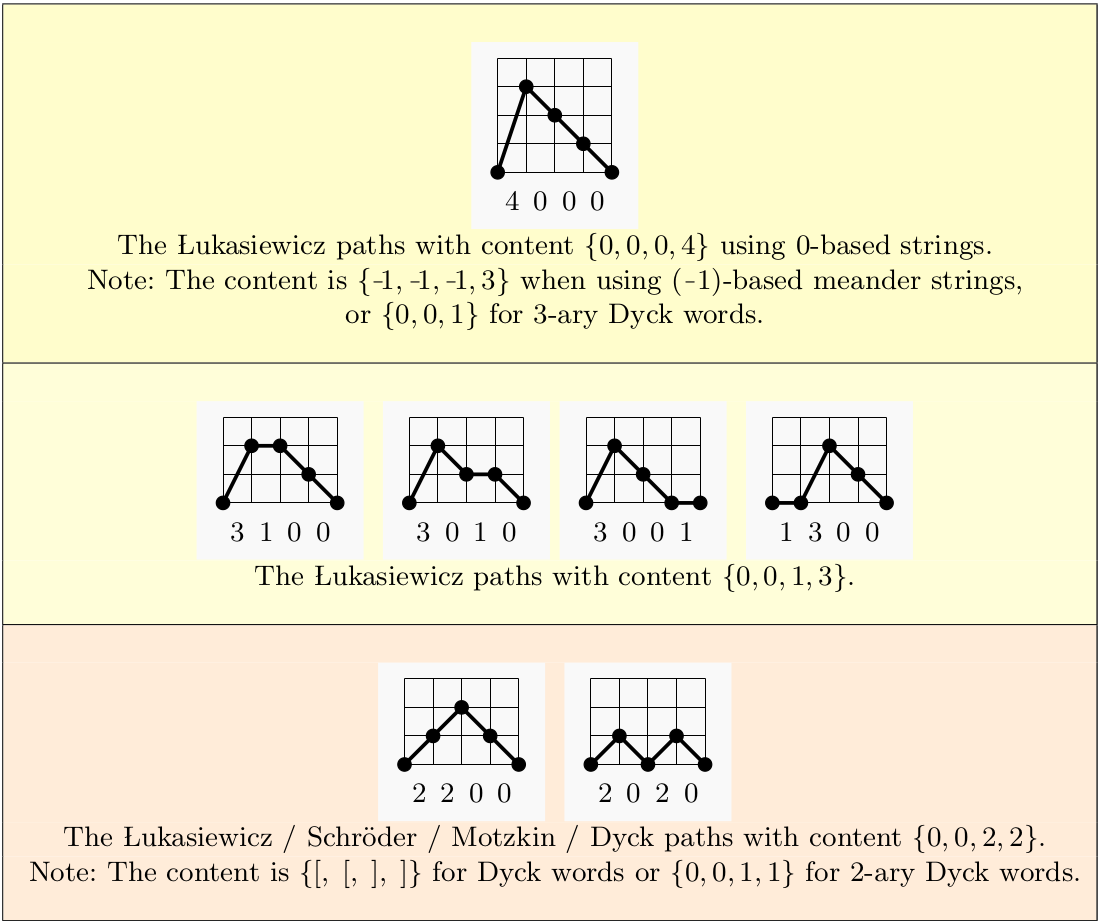
\includegraphics[width = .95 \textwidth]{paths.png}
	\caption{}
	\label{fig:paths}
\end{figure}


The number of Dyck words with n zeroes and n ones are counted by the $n$st Catalan number.  Similarly, the number of Motzkin and Schröder paths of order $n$ are counted by the $n\thh$ Motzkin and big Schröder number respectively. The number of Lukasiewicz paths of order $n$ are counted by the $n-1$st Catalan number. % TODO: is this right?
Motzkin, Schröder, and Lukasiewicz paths bear a number of interesting bijective correspondences with other combinatorial objects. Richard Stanely's \emph{Catalan Objects} outlines hundreds of interesting examples.  

Lukasiewicz paths  of order $n$ bear a particularly nice correspondence to rooted ordered trees with $n$ nodes. See Fig. \ref{trees} for an illustration of this.

\begin{figure}[]
	\centering
	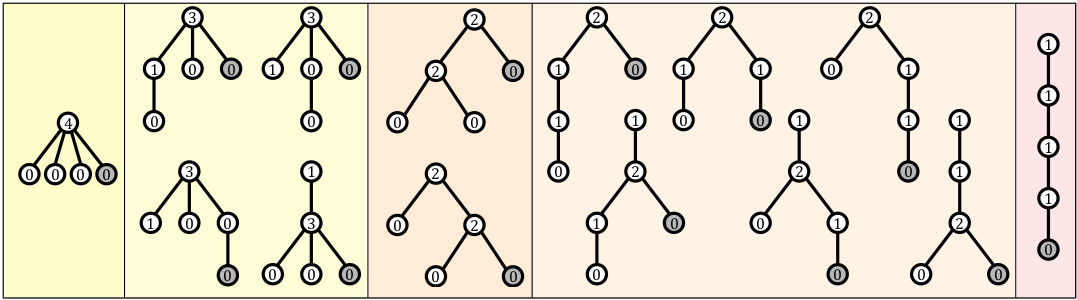
\includegraphics[width = .95 \textwidth]{trees.png}
	\caption{The $\mathcal{C}_4$=14 Lukasiewicz paths of order $n=4$ are in bijective correspondence with the 14 rooted ordered trees with $n+1=5$ nodes.  Given a tree, the corresponding word is obtained by recording the number of children of each node in preorder traversal; the zero from the rightmost leaf is omitted.  For example, the two trees in the middle section correspond to 2200 (top) and 2020 (bottom) respectively.}
	\label{trees}
\end{figure}

% TODO: bijections, mirror chapter 2

